\documentclass[11pt,a4paper]{article}
\usepackage{apacite}
\usepackage{float}
\usepackage{setspace}
\usepackage{fancyhdr}
\usepackage{natbib}
\usepackage{caption}
\usepackage{indentfirst}
\usepackage{changepage}
\usepackage[brazilian]{babel}
\usepackage[T1]{fontenc}
\PassOptionsToPackage{hyphens}{url}
\usepackage{hyperref}
\usepackage{graphicx}
\usepackage{fancyhdr}
\usepackage{times}
\usepackage{floatflt}
\usepackage{colortbl}
\usepackage{fancyvrb}
\usepackage{wrapfig}
\usepackage[utf8]{inputenc}
\newcommand{\fonte}[1]{\caption*{Fonte: {#1}} }
\usepackage{csquotes}
\usepackage{multirow}
\usepackage{siunitx}

\sisetup{
output-decimal-marker = {,},
}


%%%TORNAR TABELA AJUSTÁVEL é só usar \p{}
\newcolumntype{L}[1]{>{\raggedright\let\newline\\\arraybackslash\hspace{0pt}}m{#1}}
\newcolumntype{C}[1]{>{\centering\let\newline\\\arraybackslash\hspace{0pt}}m{#1}}
\newcolumntype{R}[1]{>{\raggedleft\let\newline\\\arraybackslash\hspace{0pt}}m{#1}}

%Margens
\setlength{\voffset}{-2.54cm}
\setlength{\hoffset}{-2.54cm}
\setlength{\textheight}{24,7cm}
\setlength{\textwidth}{17cm}
\setlength{\headwidth}{17cm}
\setlength{\parindent}{0.5cm}
\setlength{\topmargin}{1.5cm}
\setlength{\headheight}{0.5cm}

%Sections
\makeatletter
\def\section{\@startsection{section}{1}
          {\z@}{10pt minus 0pt}{10pt minus 0pt}{\bf}}
\def\subsection{\@startsection{subsection}{2}
          {\z@}{10pt minus 0pt}{10pt minus 0pt}{\bf}}
\def\subsubsection{\@startsection{subsubsection}{3}
          {\z@}{10pt minus 0pt}{10pt minus 0pt}{\bf}}
\def\thesection{\arabic{section}.\hskip -1ex}	
\def\thesubsection {\thesection\hskip 1.1ex \arabic{subsection}\hskip -1ex}
\def\thesubsubsection {\thesubsection\hskip 1.1ex .\arabic{subsubsection}\hskip -1ex}
\makeatother

\begin{document}

\thispagestyle{plain}
\pagestyle{fancy}
\setlength{\headheight}{31pt}
\rhead{	\footnotesize{\textsf{III Congresso Aeroespacial Brasileiro - CAB \\ 28 de Setembro a 1 de Outubro de 2020, Belo Horizonte, MG, Brasil}}  }
\lhead{}

% \begin{figure}
%     \centering
%     % 
\includegraphics[scale=0.83]{figures/cabecalho.pdf}
% \end{figure}

\begin{center}
\vspace{-4mm}
\Large{\textbf{USO DO NASTRAN PARA ANÁLISE DE FLUTTER SUPERSÔNICO DE PAINÉIS}}
 \end{center}
 
\hrulefill

%RESUMO
\begin{adjustwidth}{0.5cm}{0cm}

\textbf{Victor Silva dos Santos}$^{a}$; \textbf{Hélio de Assis Pegado}$^{a}$;
% \textbf{Terceito Autor}$^{c}$
\newline
[a] Universidade Federal de Minas Gerais -- Escola de Engenharia --
Departamento de Engenharia Mecânica -- Av. Presidente Antônio Carlos, 6627, Pampulha, Belo Horizonte, MG, Brasil
% \newline
% [b] Associação do autor $b$ e endereço da instituição
% \newline
% [c] Associação do autor $c$ e endereço da instituição

\hspace{0.2cm}

\noindent \textit{\textbf{Resumo}: 
O flutter de painéis é um fenômeno de grande interesse em aplicações supersônicas.
Neste trabalho a ferramenta de pré-processamento para o NASTRAN,
desenvolvida em trabalho passado, é 
utilizada para uma análise de convergência de malha, e para casos
estruturais mais complexos (i.e. placa de material composto), obtendo-se os parâmetros da fronteira de estabilidade. Os resultados apresentados mostram boa correlação com a literatura e portanto demonstram a capacidade da metodologia de análise para estes casos.
}
\end{adjustwidth}

\vspace{0.5cm}

\begin{adjustwidth}{0.4cm}{0cm}

\textit{\textbf{Palavras-chave}: painéis, aeroelasticidade, flutter, nastran, supersônico.}

\end{adjustwidth}

\hrulefill

%%%%%%%%%%%%%%%%%%%%%%%%%%%%%%%%%%%%%%%%%%%%%%%%%%%%%%%%%%%%%%%%%%%%%%%%%%%%%%%%%%%%%%%%%%%%%%%%%%%%%%%%%%%%%%%%%%%%%%%
\section{INTRODUÇÂO}

Segundo \cite{pegado_flutter_2006}, o \emph{flutter} de painéis é um
fenômeno de grande desafio e interesse no voo supersônico e 
hipersônico. Em trabalho desenvolvido anteriormente por 
\cite{santos_finite_2019}
obteve-se uma ferramenta de 
pré-processamento, geração de malha aerodinâmica e pós-processamento
para a análise aeroelástica de \emph{flutter} para o NASTRAN, um 
conjunto de códigos destinado à análise em elementos finitos 
amplamente utilizado no setor aeroespacial.

Neste artigo é primeiramente realizado um estudo das capacidades do 
MSC/NASTRAN para a modelagem 
aeroelástica e análise de \emph{flutter}.

A escolha do MSC/NASTRAN para o estudo vem de seu longo 
desenvolvimento no setor aeroespacial desde a abertura do código 
original pela NASA \citep[p. 1]{macneal_organizational_1974}, que 
hoje contém funcionalidades modernas além de
manter funcionalidades coexistentes a outros derivados do NASTRAN 
mantendo-se a reprodutibilidade do conteúdo.
Neste estudo verifica-se quais os modelos aerodinâmicos, de 
interpolação e solução do problema de autovalor de \emph{flutter} 
presente no MSC/NASTRAN.

Posteriormente, é descrito a metodologia para um estudo de 
convergência de malha e para a análise de
um caso de placa em material composto laminado, utilizando-se da Teoria Pistão.

Os resultados obtidos são discutidos e 
comparados com referências da literatura nas seções seguintes.


\section{ESTUDO DAS CAPACIDADES DO NASTRAN}

A análise de estabilidade aeroelástica no MSC/NASTRAN, utilizando-se a solução 145, possui três áreas que são requeridas a atenção do usuário: a modelagem aerodinâmica; a interpolação entre as malhas estruturais e aerodinâmicas; e o método de solução aeroelástica. Nas próximas subseções cada área é discutida com um foco no problema apresentado.

\subsection{Modelagem Aerodinâmica}

O MSC/NASTRAN possui sete métodos de obtenção das matrizes aerodinâmicas: o 
\emph{Doublet-Lattice Method} (DLM); o \emph{ZONA51} ou \emph{Harmonic Gradient Method} (HGM); o \emph{Constant Pressure Method} (CPM); o DLM com
interferência asa-fuselagem; o \emph{Mach Box Method} (MBM); o \emph{Strip Theory};
e o \emph{Piston Theory} (ou Teoria Pistão).
Todos os métodos suportam um escoamento não estacionário, se diferenciando
em relação à teoria aerodinâmica aplicada, validade de condições do escoamento,
método de discretização, dentre outros detalhes pertinentes a cada método
\citep[p. 17]{patrannastran_aeroelastic_2019}.

Um resumo das principais características de cada método está disposto na Tabela 
\ref{nastran-table}, excluindo-se o DLM com interferência asa-fuselagem, já que sua aplicação foge
ao escopo deste trabalho. 

\begin{table}[H]
\centering
\caption{Resumo de características dos métodos aerodinâmicos.}
\begin{tabular}{|c|c|c|c|}
\hline
\textbf{Método} & \textbf{Teoria Aerodinâmica}                                                          & \textbf{Discretização} & \textbf{Validade de Mach} \\ \hline
DLM             & Potencial Linearizada                                                                 & \emph{Boxes}                  & Subsônico                 \\ \hline
HGM    & \begin{tabular}[c]{@{}c@{}}Supersônico\\ Potencial Linearizada\end{tabular}           & \emph{Boxes}                  & $\num{1.2} < M < \num{3.0}$           \\ \hline
CPM             & \begin{tabular}[c]{@{}c@{}}Supersônico\\ Potencial Linearizada\end{tabular}           & \emph{Boxes}                  & $\num{1,1} < M < \num{3,0}$           \\ \hline
MBM             & \begin{tabular}[c]{@{}c@{}}Supersônico\\ Potencial Linearizada\end{tabular}           & \emph{Boxes}                  & $\num{1.2} < M < \num{3.0}$           \\ \hline
\emph{Strip Theory}    & Potencial Linearizada                                                                 & \emph{Strips}                 & Subsônico                 \\ \hline
\emph{Piston Theory}   & \begin{tabular}[c]{@{}c@{}}Pistão de 3ª Ordem\\ com correção de Van Dyke\end{tabular} & \emph{Strips}                 & $\num{2,5} < M < \num{7,0}$           \\ \hline
\end{tabular}
\fonte{\cite{liu_recent_1996} e \cite{patrannastran_aeroelastic_2019}}
\label{nastran-table}
\end{table}

Algumas características são importantes para se entender a Tabela \ref{nastran-table}.
As teorias aerodinâmicas potenciais linearizadas não levam em consideração a espessura do perfil aerodinâmico, o que não é desejável, já que a espessura tem um efeito de reduzir a velocidade de \emph{flutter}. Tal fato não ocorre no método \emph{Piston Theory} que possibilita a correção para espessura.

A discretização em \emph{Boxes} é disposta como um \emph{grid} planar de elementos retangulares
ou triangulares como indicado na Figura \ref{fig-boxes}.
Duas diferenças são notáveis: no método CPM não é possível utilizar elementos triangulares;
e no método MBM o usuário deve definir os geometria da superfície aerodinâmica e a rotina computará os elementos que, por sua vez, possuirão sua 
diagonal paralela a linha de Mach, tal como ilustrado na Figura \ref{fig-mach-boxes}.
Nestas formulações há a influência aerodinâmica entre os elementos.

\begin{figure}[H]
\centering
\caption{Discretização em \emph{Boxes}.}
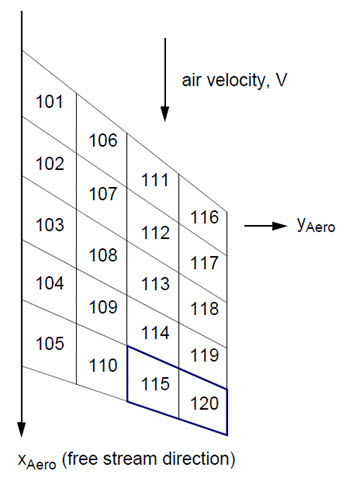
\includegraphics[width=0.4\linewidth]{figures/boxes.png}
\fonte{\cite{patrannastran_aeroelastic_2019}}
\label{fig-boxes}
\end{figure}

\begin{figure}[H]
\centering
\caption{Discretização em \emph{Boxes} para o método MBM.}
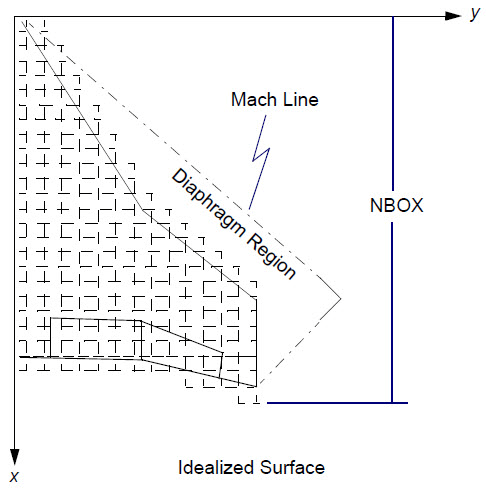
\includegraphics[width=0.5\linewidth]{figures/mach-boxes.png}
\fonte{\cite{patrannastran_aeroelastic_2019}}
\label{fig-mach-boxes}
\end{figure}

Já a discretização em \emph{Strips} (ou faixas)  é a disposição de faixas coplanares como ilustrado na Figura \ref{fig-strips}, nestas formulações não há influência aerodinâmica entre as faixas.

\begin{figure}[H]
\centering
\caption{Discretização em \emph{Strips}.}
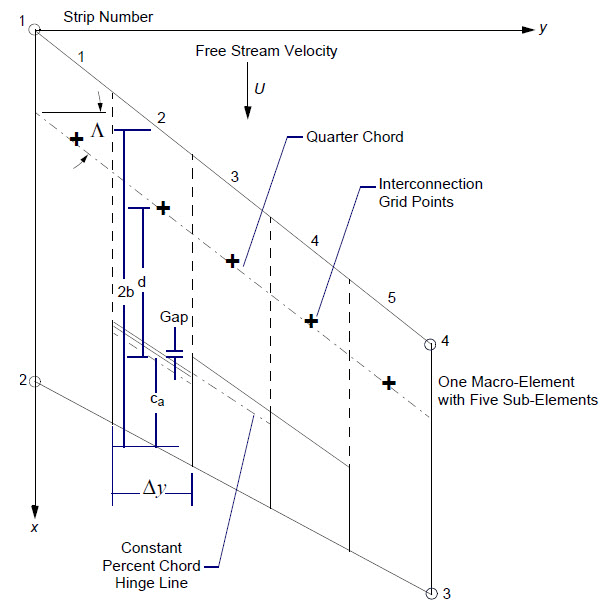
\includegraphics[width=0.5\linewidth]{figures/strip.png}
\fonte{\cite{patrannastran_aeroelastic_2019}}
\label{fig-strips}
\end{figure}

Além disto, alguns métodos possibilitam a modelagem de superfícies de controle, correções para enflechamento (\emph{sweep angle}), compressibilidade, dentre outras propriedades. Tais possibilidades não serão discutidas por fugirem do escopo deste trabalho.

Os métodos apresentam restrições quanto à sua utilização. Na Tabela \ref{nastran-table} verificamos em qual regime de número de Mach cada método se enquadra. Há também restrições de natureza geométrica: no \emph{Piston Theory} é preciso que a corda se mantenha rígida, isto é, sem deformações.

\subsection{Interpolação Aerodinâmica-Estrutural}

Para se obter as matrizes aerodinâmicas e estruturais acopladas, é necessário a interpolação entre os deslocamentos e forças nodais entre as malhas aerodinâmica e estrutural. Para tanto o MSC/NASTRAN fornece cinco métodos de interpolação, totalizando dez opções de solução, contudo, são dois os mais relevantes para o problema aqui apresentado: o \emph{Surface Spline}; e o \emph{Linear Spline}.

\begin{figure}[H]
\centering
\caption{Métodos de interpolação \emph{Surface Spline} e \emph{Linear Spline}.}
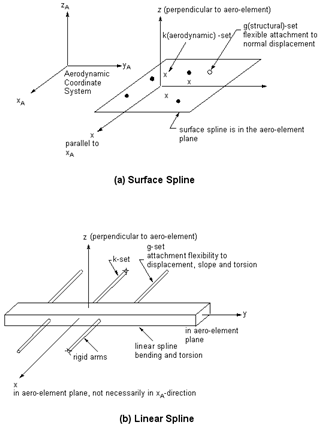
\includegraphics[width=0.6\linewidth]{figures/splines.png}
\fonte{\cite{patrannastran_aeroelastic_2019}}
\label{fig-splines}
\end{figure}

\subsection{Método de Solução Aeroelástica}

O MSC/NASTRAN fornece 6 métodos de solução aeroelástica para \emph{flutter}
o método americano \emph{K-method}; o \emph{KE-method}; o inglês \emph{PK-method}; o \emph{PKNL-method}; o \emph{PKS-method}; e o \emph{PKNLS-method}. Um resumo das características de cada método
está disposto na Tabela \ref{nastran-sol-table}.


\begin{table}[H]
\centering
\caption{Resumo de características dos métodos de solução aeroelástica.}
\begin{tabular}{|l|l|l|l|}
\hline
Método & Descrição & Entradas & Saídas \\ \hline
K      & Método iterativo americano clássico. & Conjuntos de $M$, $k$ e $\rho$   & $V$, $g$ e $f$.             \\ \hline
KE     & \begin{tabular}[c]{@{}l@{}}Variação do \emph{K-method}, desconsiderando\\ todos os amortecimentos viscosos, e com\\ uma solução somente em auto-valores.\end{tabular} & Conjuntos de $M$, $k$ e $\rho$   & $V$, $g$ e $f$.             \\ \hline
PK     & Método iterativo inglês clássico. & Combinações de $V$, $M$ e $\rho$ & $V$, $\gamma$ e $f$.         \\ \hline
PKNL   & \begin{tabular}[c]{@{}l@{}}Variação do \emph{PK-method} utilizando somente\\ conjuntos ordenados de entrada.\end{tabular}                                              & Conjuntos de $V$, $M$ e $\rho$   &$V$, $\gamma$ e $f$.         \\ \hline
PKS    & \begin{tabular}[c]{@{}l@{}}Variação do \emph{PK-method} não iterativa,\\ realizando uma "varredura" em uma faixa\\ de frequências reduzidas.\end{tabular}               & Combinações de $V$, $M$ e $\rho$ &$V$, $\gamma$ e $f$.         \\ \hline
PKNLS  & \begin{tabular}[c]{@{}l@{}}Variação do \emph{PKNL-method} não iterativa,\\ utilizando a mesma técnica do \emph{PKS-method}.\end{tabular}                                       & Conjuntos de $V$, $M$ e $\rho$   & $V$, $\gamma$ e $f$.         \\ \hline
\end{tabular}
\fonte{\cite{patrannastran_aeroelastic_2019}}
\label{nastran-sol-table}
\end{table}

Algumas comparações entre os métodos podem ser feitas.
Nos métodos tipo \emph{PK} há a inserção direta das velocidades,
o que é preferível, diferente dos métodos tipo \emph{K}, que
necessita um processo de ordenação dos resultados.
Nos métodos não iterativos, não há possibilidade de falha por
uma iteração indevida. Por fim, segundo 
\cite{rodden_mscnastran_1994}, o parâmetro de amortecimento 
$\gamma$ nos métodos tipo \emph{PK} é fisicamente mais significativo
que o parâmetro $g$ nos métodos tipo \emph{K}.

\section{METODOLOGIA}

No desenvolvimento do modelo adotou-se metodologia similar à utilizada
por \cite{santos_finite_2019}. Foram realizados melhorias do 
\emph{software}, onde passou-se a utilizar o pacote \emph{pyNastran} desenvolvido por \cite{doyle_stevedoyle2pynastran_2020},
uma ferramenta que possibilita a manipulação dos modelos com maior
facilidade. Passou-se a utilizar o cartão SET2, para facilitar a obtenção dos nós estruturais para interpolação. Estruturou-se o código afim de se tornar reutilizável para outras análises.

O software desenvolvido por \cite{santos_zuckberjnastran-aero-flutter_2020}
foi disponibilizado em repositório público com licença de tipo \emph{livre}.


\subsection{Análise de Convergência de Malha}

No estudo de convergência de malha adotou-se um modelo simples e conhecido na literatura de \emph{flutter} de painéis, uma placa retangular simplesmente apoiada, de dimensões \SI{300}{mm} de comprimento ($a$), 
\SI{300}{mm} de largura ($b$) e \SI{1.5}{mm} de espessura ($t$). O material adotado foi o alumínio.

Adotou-se um número de Mach ($M$) de \num{3}, densidade de referência ($\rho_a$) ao nível do mar ISA e corda de referência ($c_{ref}$) igual ao comprimento da placa.
Buscou-se a velocidade crítica de flutter entre \SI{822}{m/s} e \SI{1066}{m/s}, que, fixado o valor de Mach, corresponde aos valores máximos e mínimos da velocidade do som dentro da atmosfera padrão terrestre, ou seja, uma variação de altitude-densidade.

As propriedades do material adotadas foram: módulo de elasticidade ($E$) de \SI{71.7}{GPa}; módulo de cisalhamento ($G$) de \SI{26,9}{GPa}; coeficiente de Poisson ($\nu$) de \num{0,33}; e densidade ($\rho_m$) de \SI{2.81}{g/cm^3}.

Para a efeitos comparativos foram computados os valores de dois parâmetros: a pressão dinâmica adimensional ($\lambda$) dado por 

$$\lambda = \frac{2 \bar{q} a^3 }{\beta D}$$

onde
$\bar{q} = \frac{1}{2} \rho_a V^2$
é a pressão dinâmica do escoamento,
$D = E t^3/12(1 - \nu^2)$
é a rigidez à flexão da placa,
$\beta = \sqrt{M^2 - 1}$
, e $V$ é o módulo da velocidade do escoamento;
e a razão de densidades pelo número de Mach $\mu / M$ onde,
$\mu = \rho_a a/\rho_m t$ é a razão de densidades.

Calculou-se também as duas primeiras frequências de vibração teóricas
para a placa, sendo a primeira frequência $f_1$ dada por
$$f_1 = \frac{\pi}{a^2}\sqrt{\frac{D}{\rho_m t}}$$
e a segunda frequência $f_2$ dada por
$f_2 = \frac{5}{2}f_1$.

Para o tamanho de malha inicial adotou-se 10x10 elementos aerodinâmicos e estruturais, tendo por base o modelo \emph{HA145HA} analisado em \cite{rodden_mscnastran_1994}. Analisou-se então $N$ múltiplos desta malha.

É também possível analisar configurações em que os tamanhos de malha aerodinâmica e estrutural não são os mesmos. Entretanto recaímos em alguns problemas.

No caso em que a malha aerodinâmica é menor que a estrutural temos 
mais que dois nós estruturais pertencentes à região que o elemento 
aerodinâmico ocupa em uma mesma coordenada $y$. Caso fossem 
selecionados todos os nós, teríamos o desenvolvimento de uma
matriz singular, o que inviabiliza a solução. Uma alternativa seria 
utilizar valores maiores que zero para o parâmetro $D_z$ de 
\emph{displacement attachment}, o que significa que a interpolação não
necessariamente passa por todos os pontos designado, como descrito por \cite{rodden_mscnastran_1994}, entretanto esta 
alternativa viola a hipótese de corda rígida da teoria pistão e leva a
resultados insatisfatórios. Caso fossem selecionados somente uma 
parcela dos nós, haveria uma perda de representatividade física, já 
que o deslocamento dos nós não selecionados não implicaria em uma 
mudança nos nós aerodinâmicos.

Para o caso em que a malha aerodinâmica é maior que a estrutural temos
uma limitação de a malha aerodinâmica ser o dobro da malha estrutural,
isto já que para múltiplos maiores haveriam painéis aerodinâmicos 
centrais sem nós estruturais correspondentes, e, mesmo que fossem 
ligados aos nós estruturais adjacentes, não melhorariam a qualidade do
modelo já que seus deslocamentos seriam iguais aos dos painéis vizinhos.

Em casos de refinamento da malha aerodinâmica longitudinalmente não há uma melhora no resultado, já que a teoria pistão empregada é discretizada em faixas, e não há influência aerodinâmica de entre elas. Além disto, para placas quadradas, o uso de malhas com valores não simétricos, isto é, quantidade de elementos diferente nos sentidos longitudinal e lateral, não é adequado, já que pode produzir erros na solução da análise modal.

Os valores de referência foram interpolados para a comparação.

\subsection{Análise de Placa em Material Composto}

O modelo adotado foi de mesma geometria e condições de contorno de que o modelo de estudo de convergência. O material utilizado para o laminado composto foi o \emph{Glass-Epoxy} (GFRP) de propriedades descritas na Tabela \ref{tab-cfrp}. As camadas foram dispostas seguindo a metodologia descrita por \cite{}, conforme a Tabela \ref{tab-camadas}. O ângulo de orientação $\theta$ para as camadas do laminado foi variado de \SI{0}{\degree} até \SI{90}{\degree} com passo de \SI{10}{\degree}. As escolhas de propriedades do material e disposição das camadas foram arbitrariamente escolhidas para comparação com \cite{sawyer_flutter_1977}.

\begin{table}[H]
\centering
\caption{Propriedades do material GFRP.}
\begin{tabular}{|c|c|c|c|c|}
\hline
$E_1$ (\si{GPa}) & $E_2$ (\si{GPa}) & $G_{12}$ (\si{GPa}) & $\nu$ & $\rho_m$ (\si{g/cm^3}) \\ \hline
\num{54} & \num{18} & \num{7.2} & \num{0.3} & \num{2.6} \\ \hline
\end{tabular}
\label{tab-cfrp}
\end{table}

\begin{table}[H]
\centering
\caption{Disposição das camadas do laminado.}
\begin{tabular}{|c|c|c|}
\hline
Camada & Orientação (\si{\degree}) & Espessura (\si{mm}) \\ \hline
1      & $\theta$   & \num{0.5}   \\ \hline
2      & $-\theta$  & \num{0.5}   \\ \hline
3      & $-\theta$  & \num{0.5}   \\ \hline
4      & $\theta$   & \num{0.5}   \\ \hline
\end{tabular}
\label{tab-camadas}
\end{table}

Os propriedades do escoamento seguiram as mesmas da análise de 
convergência, entretanto, com um valor de $M = \num{2}$ e o 
\emph{range} de velocidades adequado.

% \subsection{Análise de Placa Quadrada com Reforçador Longitudinal}

\section{RESULTADOS}

\subsection{Convergência de Malha}

\begin{table}[H]
\centering
\caption{Resultado da análise de convergência de malha.}
\begin{tabular}{|c|c|c|c|c|} 
\hline
Tamanho de Malha & $\lambda_{critico}$ & DOF  & 1ª Frequência (\si{Hz}) & 2ª Frequência (\si{Hz}) \\ \hline
10x10            & \num{524,34}    & \num{606}  & \num{79,80}         & \num{198,50}        \\ \hline
20x20            & \num{518,67}    & \num{2406} & \num{80,48}         & \num{200,92}        \\ \hline
30x30            & \num{517,81}    & \num{5406} & \num{80,64}         & \num{201,49}        \\ \hline
40x40            & \num{517,07}    & \num{9606} & \num{80,69}         & \num{201,70}        \\ \hline
\end{tabular}
\label{tab-result-conv}   
\end{table}

Analisando-se quatro casos com $N$ de 1 até 4 obteve-se os valores
dispostos na tabela \ref{tab-result-conv} de $\lambda$, graus de
liberdade estimados do modelo (DOF), e as duas primeiras frequências
de vibração computadas.


Os erros comparados com a literatura estão dispostos na tabela 
\ref{tab-result-conv-comp}.
Foram utilizados os parâmetros $\beta a/b = \num{2,83}$ e $\mu/M = 
\num{0,0291}$ para a interpolação dos valores das tabelas de
\cite{hedgepeth_flutter_1957} e \cite{pegado_metodo_2003}, 
respectivamente, obtendo-se os valores de $\lambda$ de \num{496,19} e 
\num{515,15}, respectivamente. Os valores teóricos das frequências são
$f_1 = \SI{80.88}{Hz}$ e $f_2 = \SI{202.20}{Hz}$

\begin{table}[H]
\centering
\caption{Resultado comparativo da convergência de malha com a literatura.}
\begin{tabular}{|c|c|c|c|c|}
\hline
\multirow{2}{*}{Tamanho de Malha} & \multicolumn{4}{c|}{Erro Percentual}                 \\ \cline{2-5} 
                                  & Hedgepeth (1957) & Pegado (2003) & $f_1$   & $f_2$   \\ \hline
10x10                             & \SI{5.67}{\percent}           & \SI{1.78}{\percent}         & \SI{-1.34}{\percent}  & \SI{-1.83}{\percent}  \\ \hline
20x20                             & \SI{4.53}{\percent}           & \SI{0.68}{\percent}         & \SI{-0.50}{\percent}  & \SI{-0.64}{\percent}  \\ \hline
30x30                             & \SI{4.36}{\percent}           & \SI{0.52}{\percent}         & \SI{-0.30}{\percent}  & \SI{-0.35}{\percent}  \\ \hline
40x40                             & \SI{4.21}{\percent}           & \SI{0.37}{\percent}         & \SI{-0.24}{\percent}  & \SI{-0.25}{\percent}  \\ \hline
\end{tabular}
\label{tab-result-conv-comp}
\end{table}

\subsection{Placa em Material Composto}

Utilizando-se a malha 20x20 realizou-se a análise obtendo-se os 
valores de $\lambda$ em função de $\theta^*$, comparados com o 
resultado obtido por \cite{sawyer_flutter_1977}, conforme a Figura 
\ref{fig-result-comp}. O parâmetro $\lambda^*$ é semelhante ao 
utilizado anteriormente, entretanto, como a rigidez à flexão da 
placa se torna matricial devido a natureza do material composto, 
utiliza-se $\bar{D}_{11}$ com $\theta = 0$ como valor de referência.
O valor de $\bar{D}_{11}$ pode ser computado facilmente na maioria 
dos \emph{softwares} que suportam análise de laminados.

\begin{figure}[H]
\centering
\caption{Valores de pressão dinâmica adimensional crítica em função da orientação do material.}
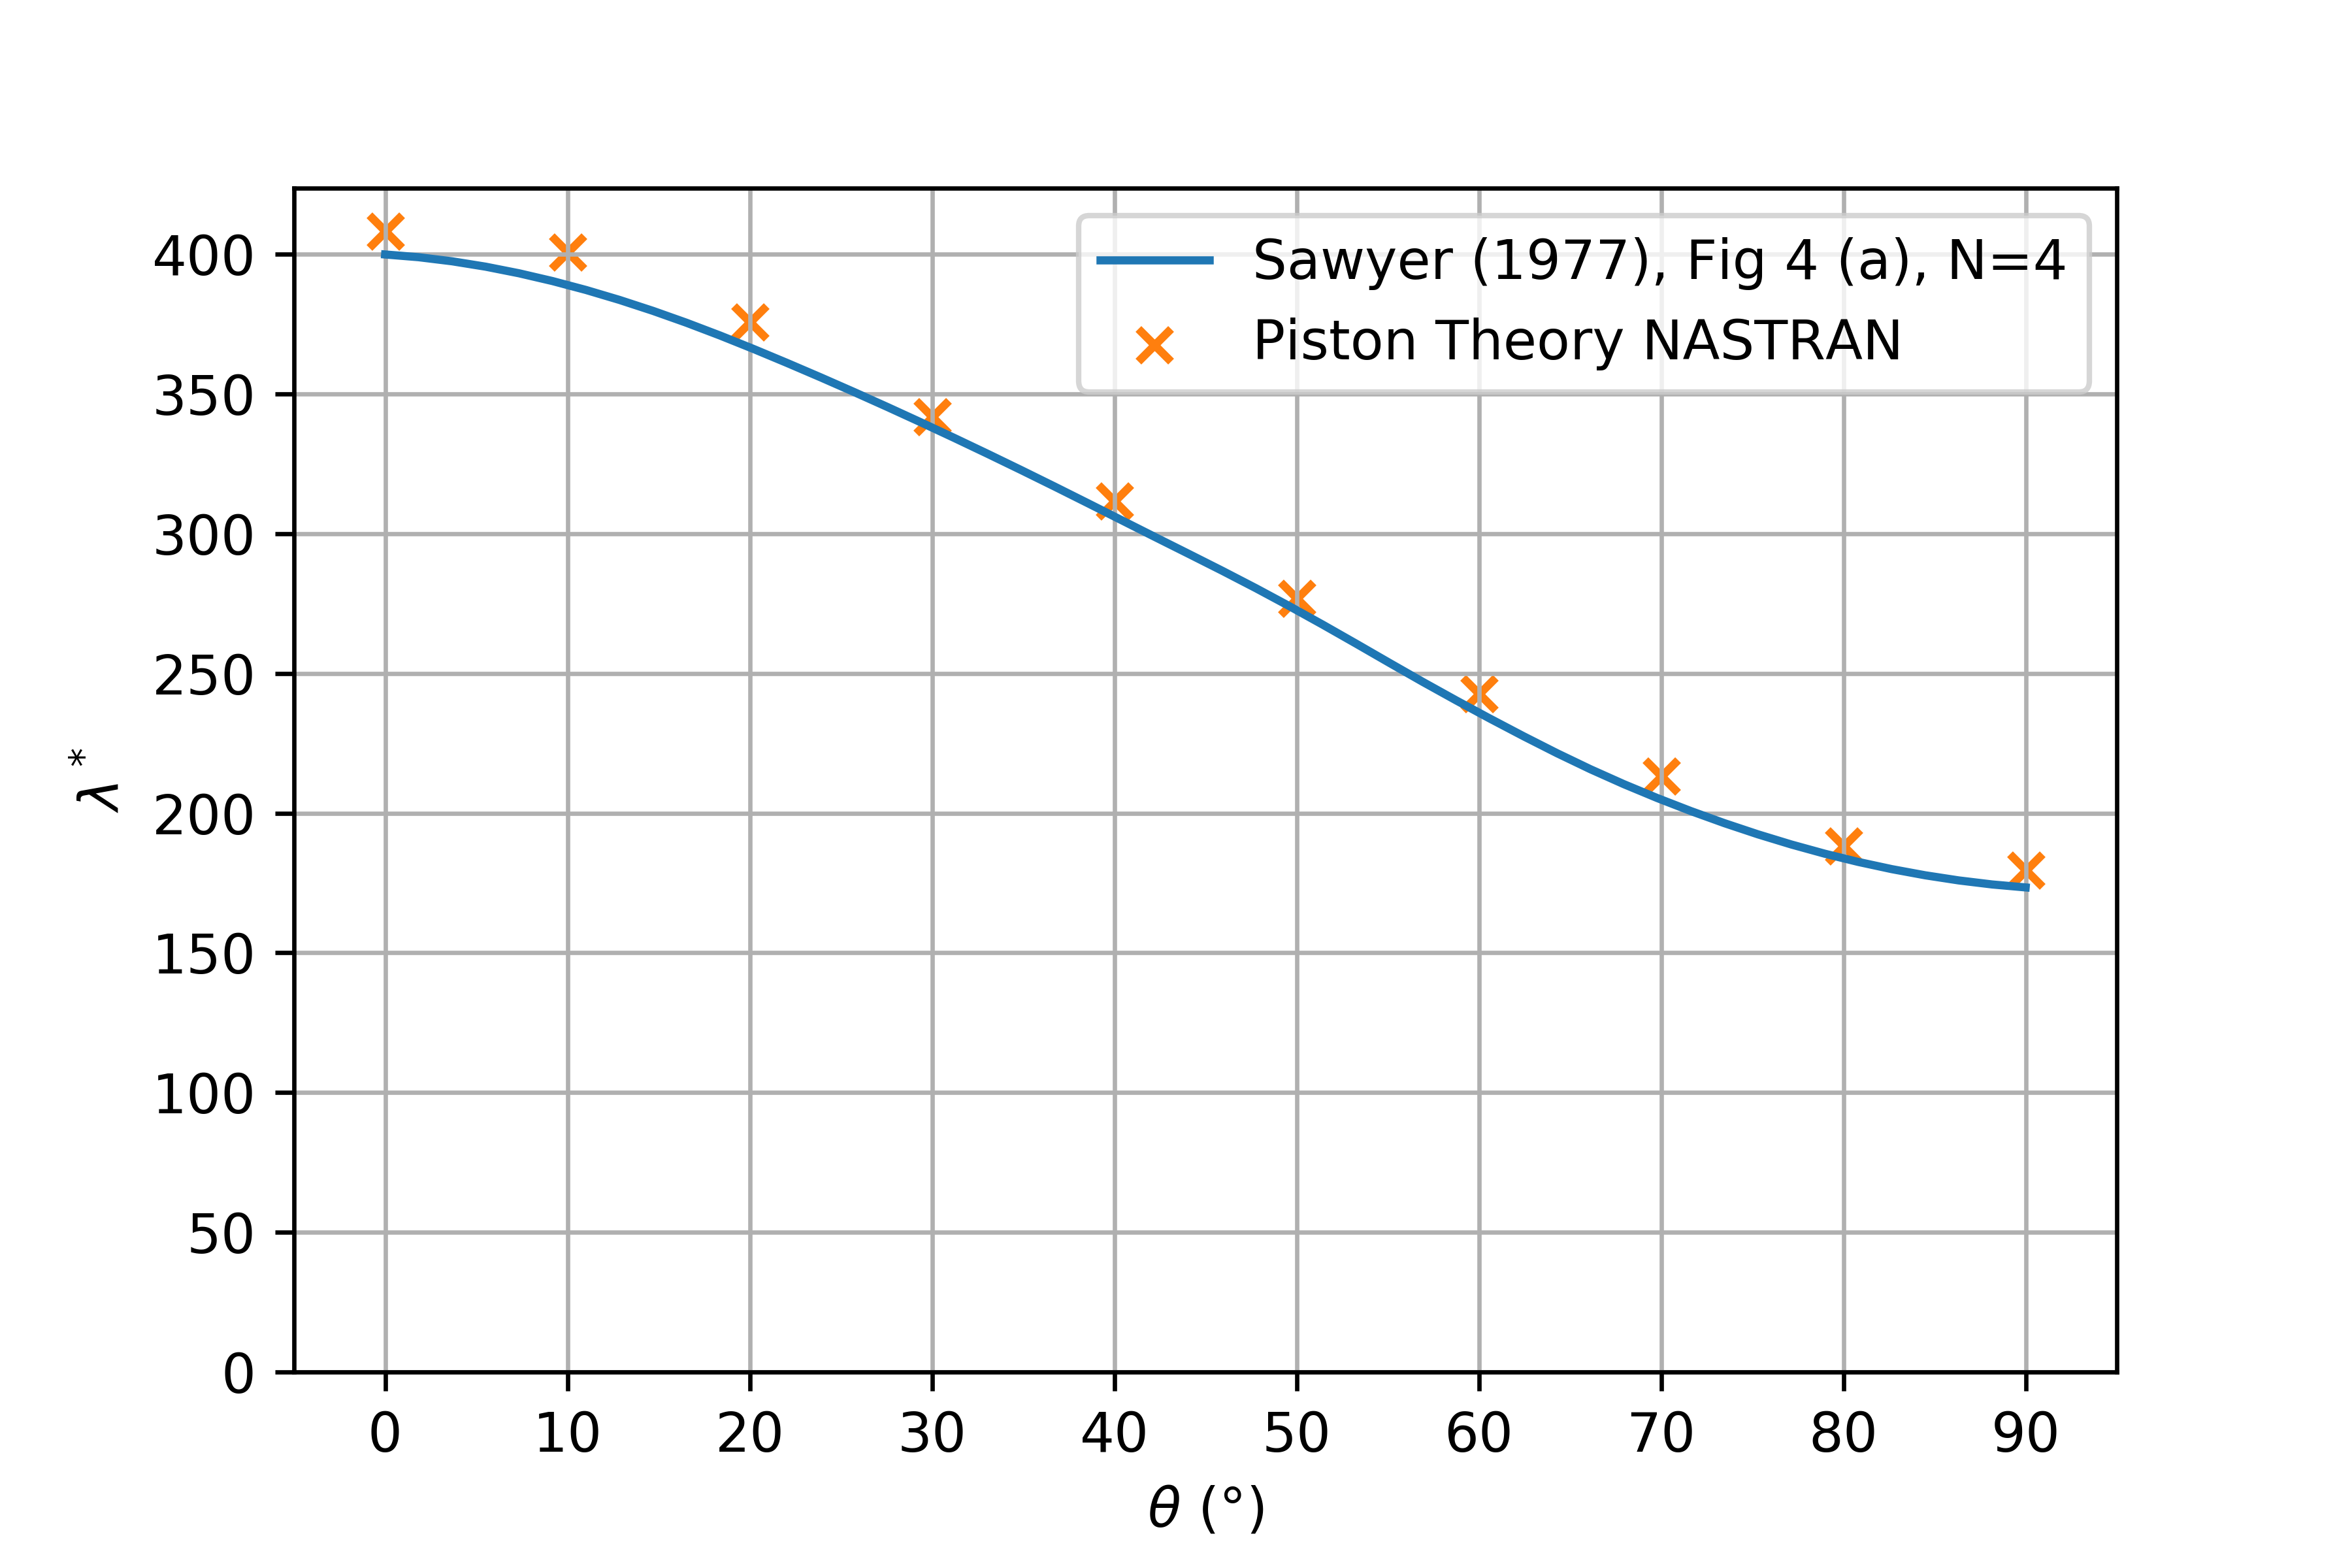
\includegraphics[width=0.7\linewidth]{figures/reference-77.png}
% \fonte{\cite{cook}.}
\label{fig-result-comp}
\end{figure}

% \subsection{Placa Quadrada com Reforçador Longitudinal}

\section{DISCUSSÕES}

Na análise de convergência de malha obteve-se resultados 
satisfatórios com a malha 20x20, tendo um erro menor que 
\SI{1}{\percent}, convergindo "por cima" para o valor de referência 
de \cite{pegado_metodo_2003}, o que está dentro do próprio erro 
indicado pela referência, que, por sua vez, converge "por baixo" aos
valores indicados por \cite{dowell_aeroelasticity_1974}. Para os valores 
encontrados por \citet[Table 2]{hedgepeth_flutter_1957} temos um 
erro menor que $5\%$ convergindo "por cima".

Para malhas com maiores números de elementos houve pouco ganho de precisão, enquanto houve um aumento significativo na quantidade de graus de liberdade e por consequência um aumento no gasto computacional.

É possível inferir que há uma correlação entre a precisão das frequências dos primeiros modos de vibração com a precisão de $\lambda_{critico}$.
O que é de se esperar, já que, usualmente, o acoplamento dos dois primeiros modos gera o caso de \emph{flutter} mais crítico, e portanto, a precisão com que os primeiros modos são representados no modelo em FEM impacta diretamente o resultado.

Sendo assim, o uso de uma malha 20x20 é encorajado, já que fornece boa precisão com relativo baixo custo computacional. Pode-se sugerir que em configurações onde $a \neq b$ ou exista assimetria, outros valores de malha sejam usados com outros fins (e.g. manter a razão de aspecto do elemento adequada), mas que se mantenham um mínimo de 20 elementos em cada dimensão.

A metodologia aplicada no problema de painel composto se mostrou suficientemente próxima à referência, observando-se a mesma tendência e com erros menores que \SI{5}{\percent}, entretanto convergindo "por cima", o que indica uma tendência não conservadora do modelo.



\section{CONCLUSÃO}

Neste trabalho aplicou-se a metodologia de trabalhos previamente 
desenvolvidos, onde se obteve um valor desejado de malha para a 
análise.
Ainda, aplicando-se o modelo em uma estrutura de maior complexidade 
como um painel de material composto, obteve-se resultados próximos aos 
encontrados na literatura, entretanto, todos os casos se mostraram não 
conservadores.

Como demonstrada a aplicabilidade da metodologia, é possível a análise em estruturas geometricamente similares, com diferentes materiais, e estruturas adjacentes (e.g. reforçadores), sem em maiores dificuldades. Todavia, a análise em outros casos de geometria não plana (e.g. painéis curvos, cascas) podem vir a levar outras problemáticas e um novo desenvolvimento da metodologia.














\bibliographystyle{apacite}
\bibliography{bibliography}

\end{document}

